FedMATRIX-LoRA 通过客户端相关评估与资源可行分配实现重要性引导的矩阵选择。图~\ref{fig:overview} 区分了这两个作用。客户端利用本地数据对当前适配器进行画像，形成可独立选择目标的配置。服务器在轮次预算和时延目标下协调这些配置。随后，客户端更新被分配的因子，各客户端的贡献按矩阵聚合为下一轮共享适配器。以下小节分别说明评分规则、分配过程、训练协议与条件性分析。

\begin{figure*}[!t]
  \centering
  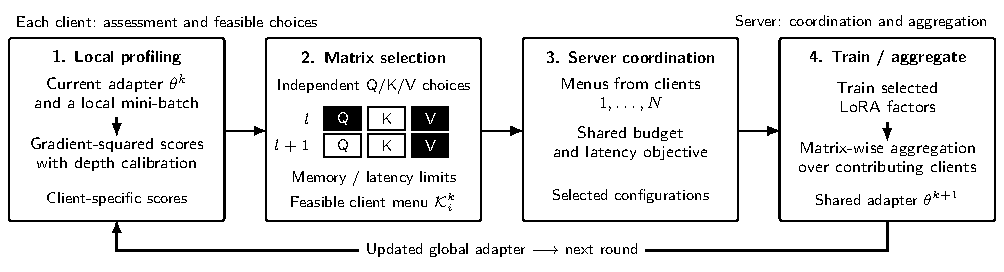
\includegraphics[width=.98\textwidth]{figures/fig2_method_overview_p2.pdf}
  \caption{FedMATRIX-LoRA 工作流程。本地梯度画像指导独立的目标投影选择。客户端配置生成施加内存和时延约束；服务器在共享轮次预算下选择配置。客户端更新被分配的 LoRA 因子，按矩阵聚合得到下一轮全局适配器。图中的 Q/K/V 子集仅作示意，不代表实验中的实际选择。}
  \label{fig:overview}
\end{figure*}
